% This example is meant to be compiled with lualatex or xelatex
% The theme itself also supports pdflatex
\PassOptionsToPackage{unicode}{hyperref}
\documentclass[aspectratio=1610, 9pt, xcolor=dvipsnames]{beamer}
\usepackage{graphicx,caption}
\parskip0pt
% Load packages you need here
\usepackage{polyglossia}
\setmainlanguage{german}

\usepackage{csquotes}

\usepackage{tikz}

\usepackage{subfig}

\usepackage[export]{adjustbox}

\usepackage{amsmath}
\usepackage{amssymb}
\usepackage{mathtools}

\usepackage{hyperref}
\usepackage{bookmark}
\usepackage{graphicx}
\usepackage{wrapfig}

\usepackage{booktabs}

\usepackage{multicol}

\usepackage{relsize}

\usepackage[dvipsnames]{xcolor}

\usepackage{empheq}
\newcommand*\widefbox[1]{\fbox{\hspace{2em}#1\hspace{2em}}}

\makeatletter
\newcommand{\Pause}[1][]{\unless\ifmeasuring@\relax
\pause[#1]%
\fi}
\makeatother

\usepackage[
locale=DE,
separate-uncertainty=true, % Immer Unsicherheit mit ±
per-mode=symbol-or-fraction, % m/s im Text, sonst \frac
% alternativ:
% per-mode=reciprocal, % m s^{-1}
% output-decimal-marker=., % . statt , für Dezimalzahlen
]{siunitx}

% load the theme after all packages

\usetheme[
  showtotalframes, % show total number of frames in the footline
]{tudo}

% Put settings here, like
\unimathsetup{
  math-style=ISO,
  bold-style=ISO,
  nabla=upright,
  partial=upright,
  mathrm=sym,
}

\DeclarePairedDelimiter{\bra}{\langle}{\rvert}
\DeclarePairedDelimiter{\ket}{\lvert}{\rangle}
\DeclarePairedDelimiterX{\braket}[2]{\langle}{\rangle}{
#1 \delimsize| #2
}

%----------------------------------------
%Align Equations to LEFT MARGIN (use \mathleft then \mathcenter)
\makeatletter
\newcommand{\mathleft}{\@fleqntrue\@mathmargin0pt}
\newcommand{\mathcenter}{\@fleqnfalse}
\makeatother
%----------------------------------------

\title{Mid-Infrared Instrument cryocooler}
\author[Y.~Kind]{Yanick Kind}
\institute[SoAk22]{Sommerakademie 2022}
\date{15. September 2022}
%\titlegraphic{\includegraphics[width=0.7\textwidth]{images/tudo-title-2.jpg}}


\begin{document}

\maketitle

%\begin{frame}{Übersicht}
%  \begin{columns}
%    \column{0.4\linewidth}
%    \setlength{\parskip}{4ex}
%    \tableofcontents
%    \column{0.6\linewidth}
%    \vspace*{1cm}
%    \centering
%  \end{columns}
%\end{frame}

\begin{frame}{Problemstellung}
  \begin{columns}
    \column{0.3\linewidth}
    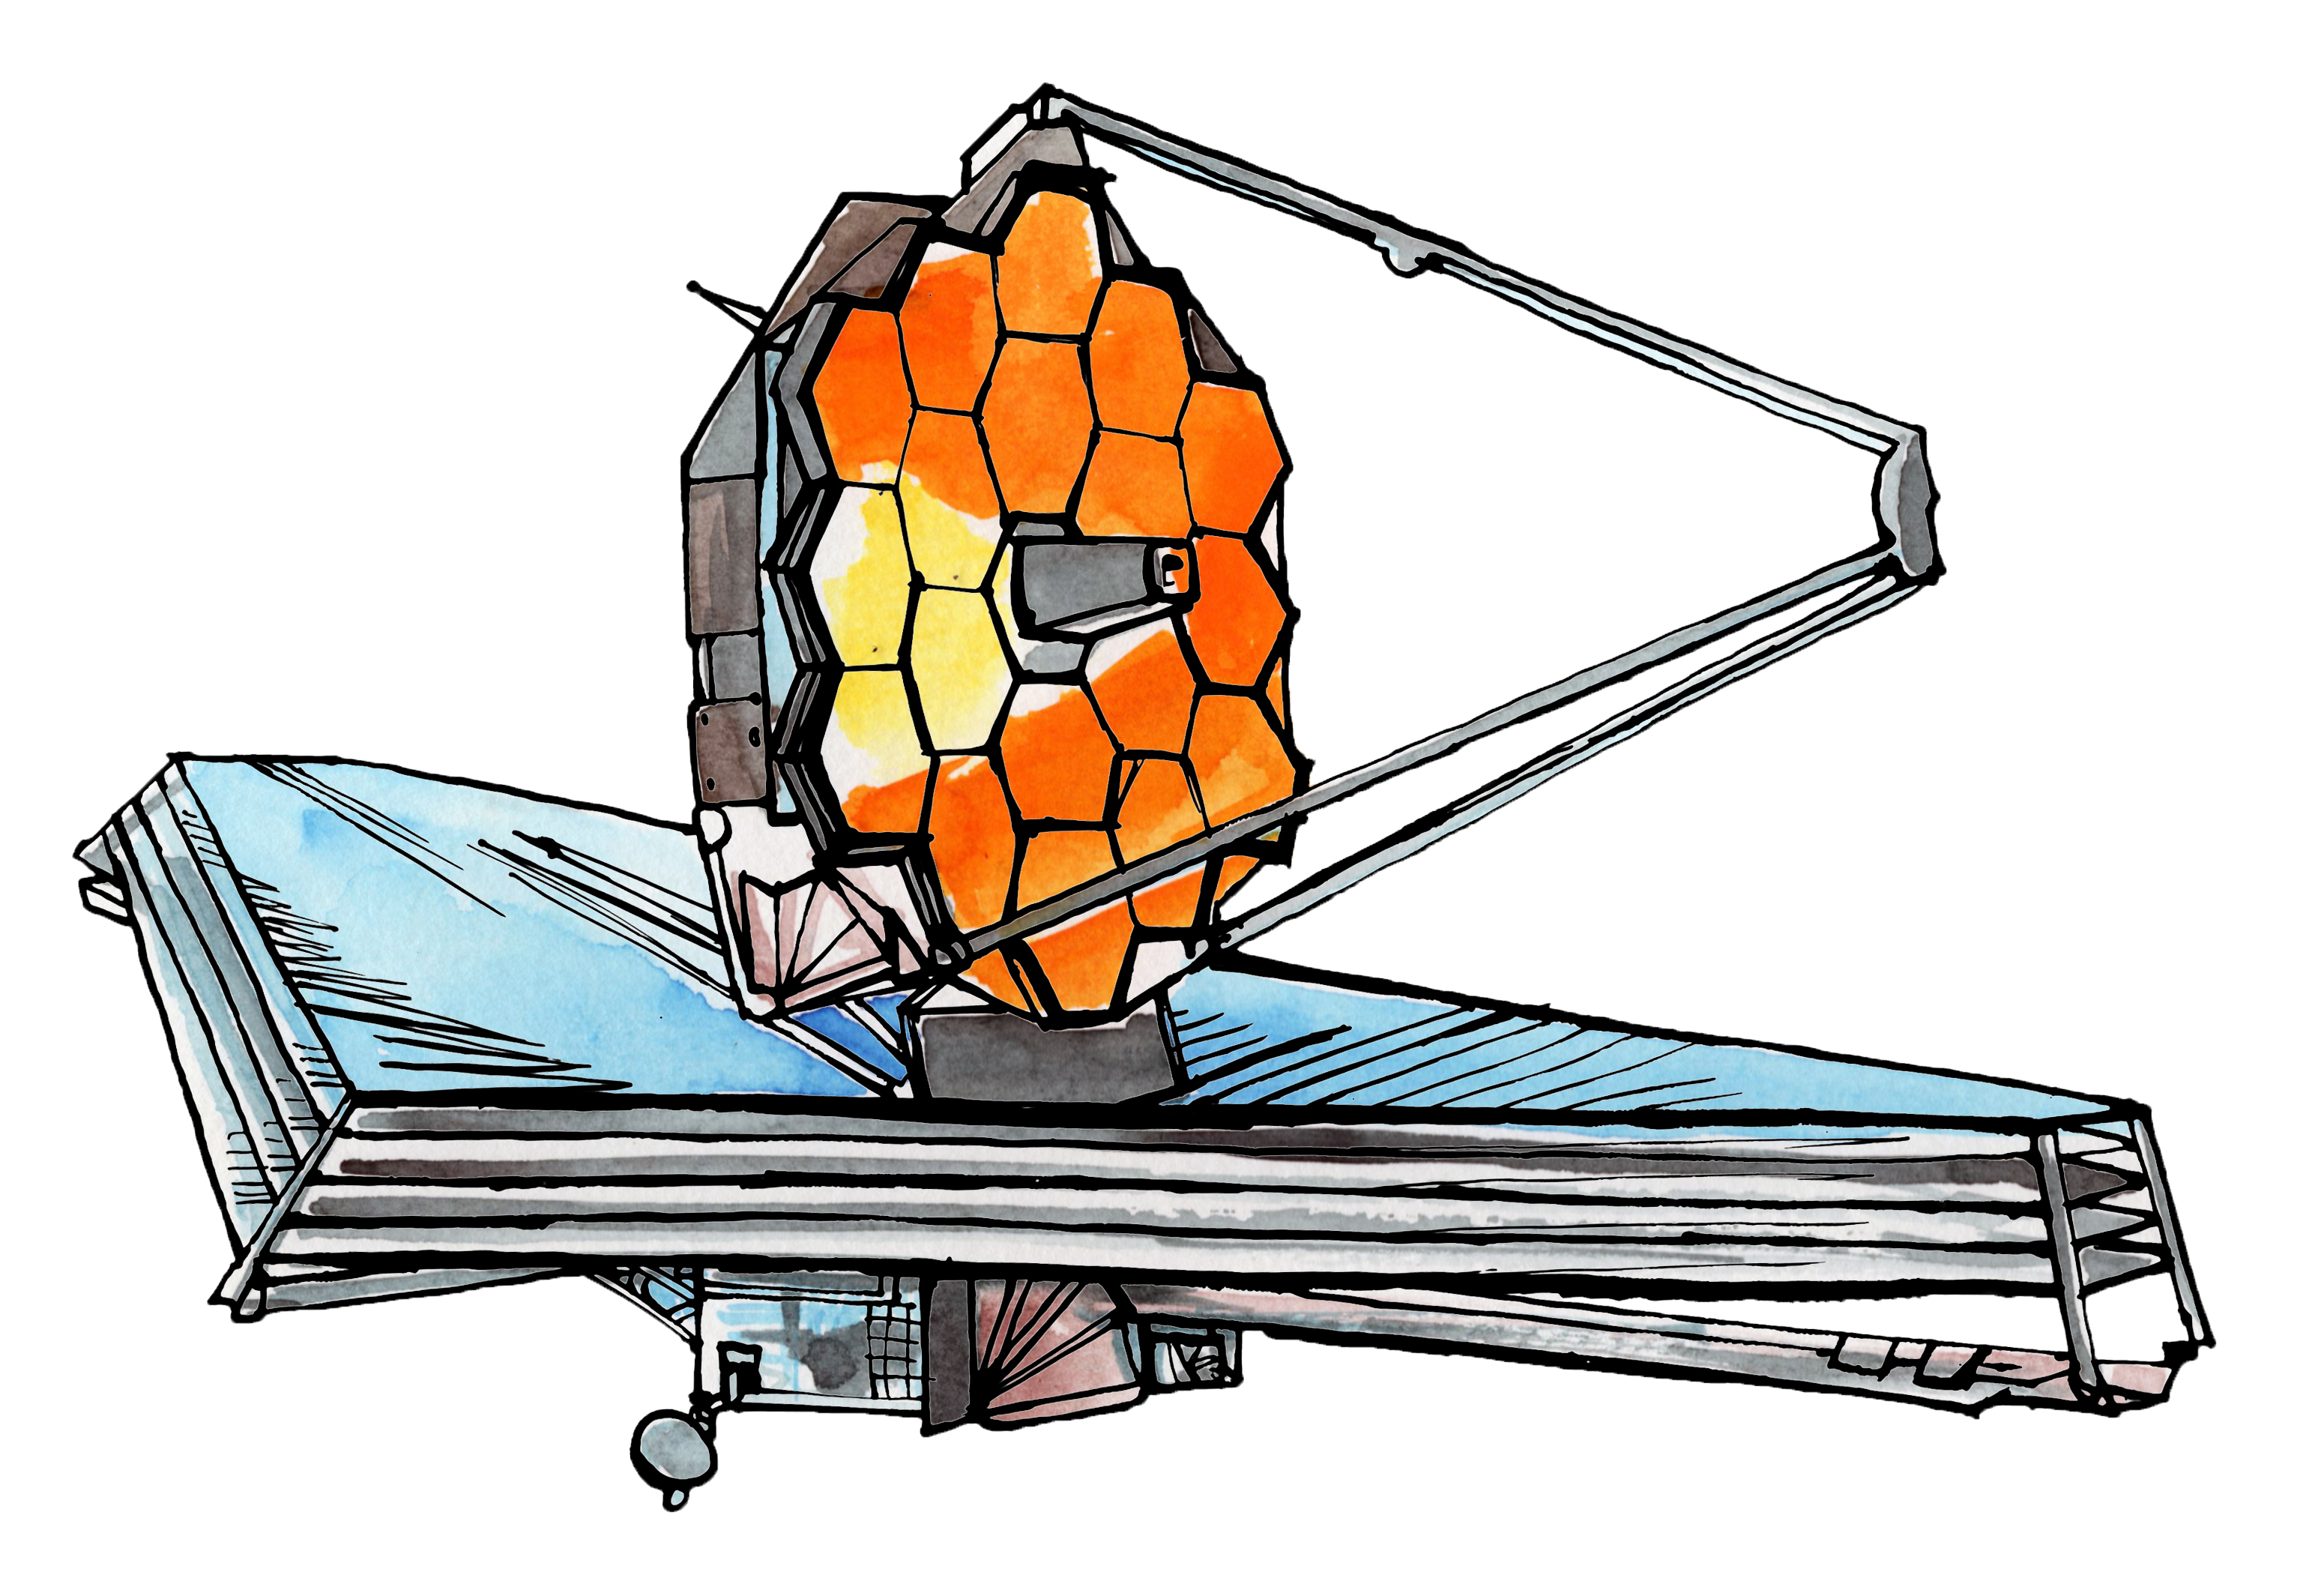
\includegraphics[width = \textwidth]{Plots/sketch.png}
    \hspace*{12pt}\hbox{\scriptsize {\footnotesize\itshape \href{https://archive.stsci.edu/missions-and-data/jwst}
    {archive.stsci.edu/missions-and-data/jwst}}}
    \column{0.7\linewidth}
  \begin{itemize}
    \item drei von vier Messinstrumenten durch Sonnenschielde gekühlt 
    \begin{itemize}
      \item bestehen aus HgCdTe {\color{tugreen} \textrightarrow } ca. $\qty{37}{\kelvin}$
      \item messen bei $\qty{0.6}{\micro\metre}$ bis $\qty{5}{\micro\metre}$
    \end{itemize}
    \pause
    \item Mid-infrared Instrument (MIRI) misst bei $\qty{5}{\micro\metre}$ bis $\qty{28}{\micro\metre}$
    \begin{itemize}
      \item besteht aus Si:As {\color{tugreen} \textrightarrow } $<$ $\qty{7}{\kelvin}$
    \end{itemize}
  \end{itemize}
  \pause
  \vspace{0.5cm}
  \centering
  \framebox{\color{tugreen} \huge \textbf{Aktive Kühlung benötigt}}
\end{columns}
\end{frame}
\begin{frame}{Was ist MIRI?}
  \begin{itemize}
    \item misst bei $\qty{5}{\micro\metre}$ bis $\qty{28}{\micro\metre}$ (Infrarot)
    \item "sieht" rotverschobenes Licht von weit entfernten Galaxien, entstehenden Sternen, Kometen und dem Kuipergürtel
    \item Kamera liefert breitbandige Weitfeld-Aufnahmen
    \item Spektrograf liefert mittelmäßig aufgelöste Aufnahmen über ein kleines Feld
  \end{itemize}
  \begin{columns}
    \column{0.33\linewidth}
    \centering
    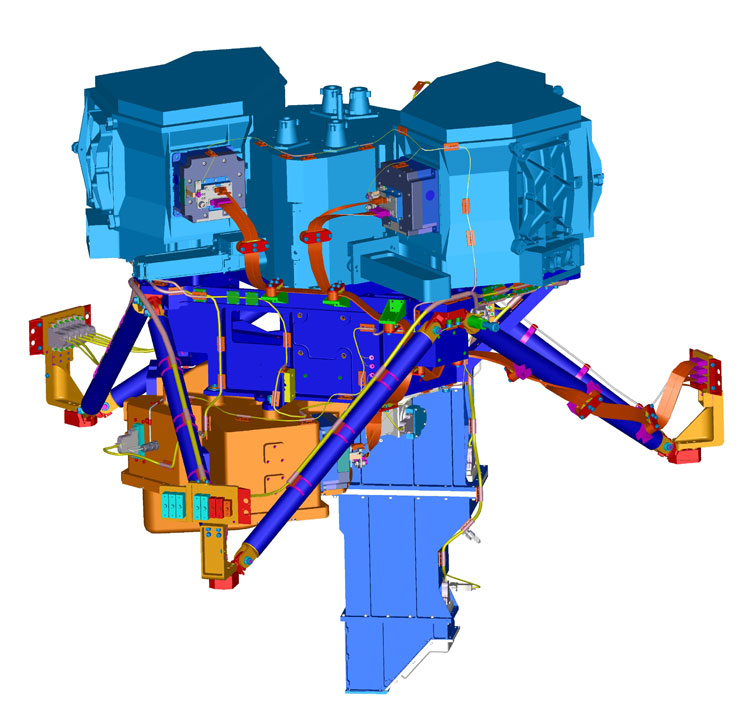
\includegraphics[width = 0.9\textwidth]{Plots/miri_cad.jpg}
  \hspace*{12pt}\hbox{\scriptsize {\footnotesize\itshape \href{https://webb.nasa.gov/content/observatory/instruments/miri.html}
  {webb.nasa.gov}}}
    \column{0.33\linewidth}
    \centering
    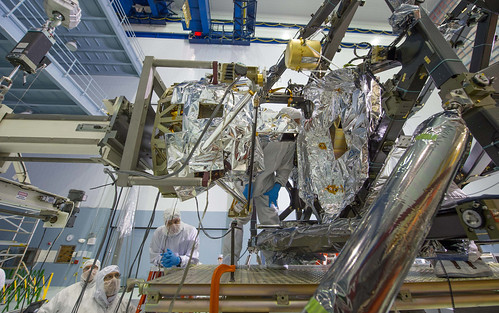
\includegraphics[width = 0.9\textwidth]{Plots/miri_installation.jpg}
  \hspace*{12pt}\hbox{\scriptsize {\footnotesize\itshape \href{https://webb.nasa.gov/content/observatory/instruments/miri.html}
  {webb.nasa.gov}}}
  \column{0.33\linewidth}
  \centering
    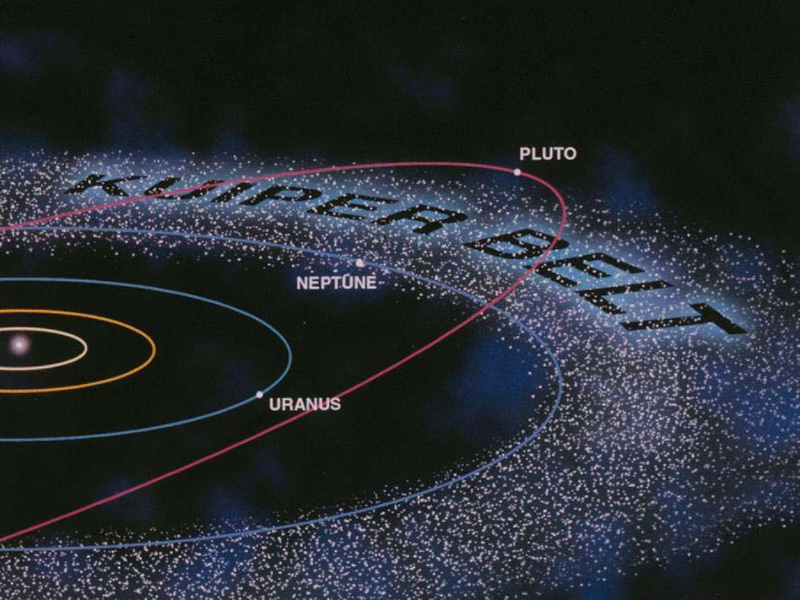
\includegraphics[width = 0.9\textwidth]{Plots/kuper.jpg}
  \hspace*{12pt}\hbox{\scriptsize {\footnotesize\itshape \href{https://solarsystem.nasa.gov/news/792/10-things-to-know-about-the-kuiper-belt/}
  {solarsystem.nasa.gov}}}
  \end{columns}
\end{frame}
\begin{frame}{Grobe Position}
  \centering
  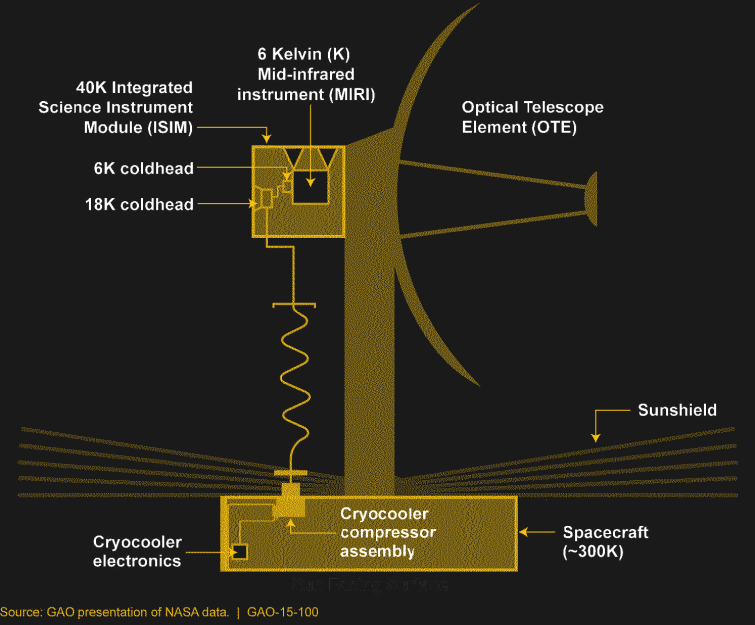
\includegraphics[width=0.5\textwidth]{Plots/position.png}
  \hspace*{12pt}\hbox{\scriptsize {\footnotesize\itshape \href{https://www.youtube.com/watch?v=FUH61gx149c}
  {youtube.com}}}
\end{frame}
\begin{frame}{Grobe Funktionsweise}
  \centering
  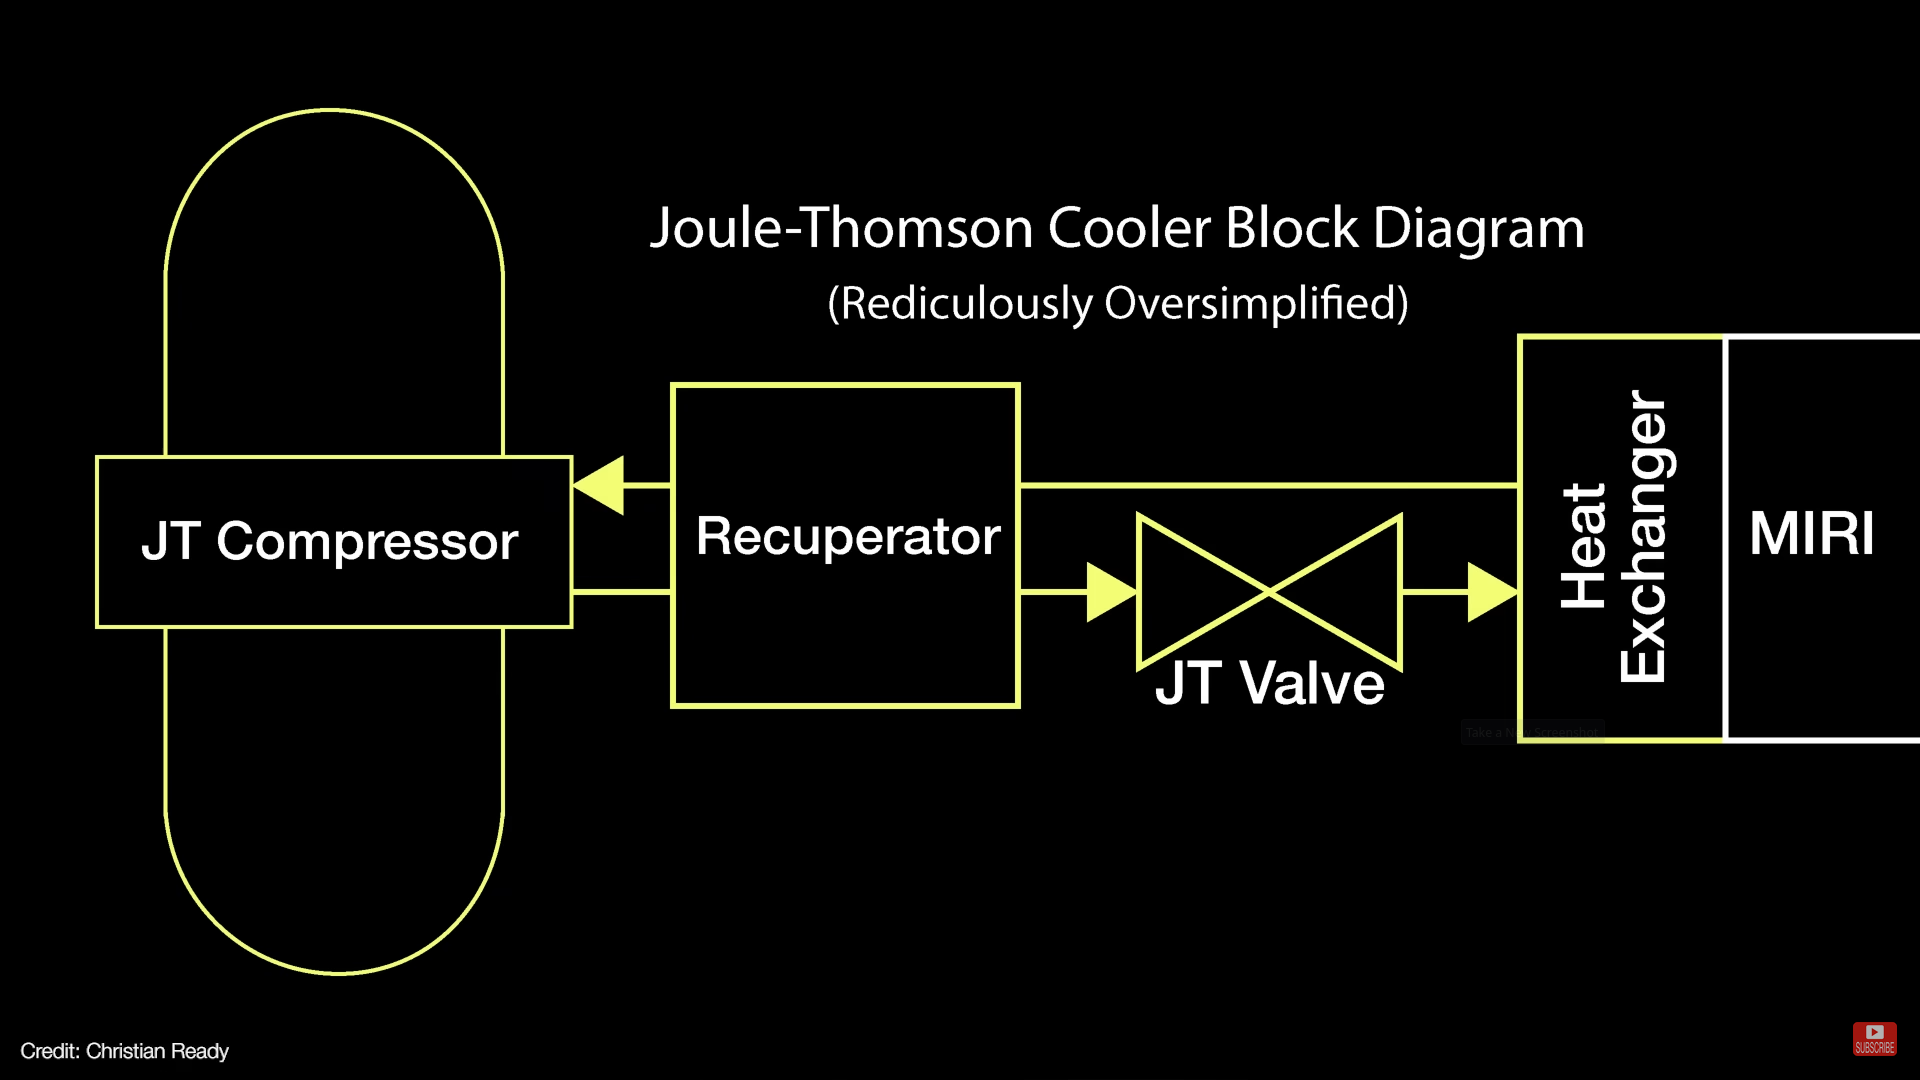
\includegraphics[width=0.85\textwidth]{Plots/grober_aufbau.png}
  \hspace*{12pt}\hbox{\scriptsize {\footnotesize\itshape \href{https://www.youtube.com/watch?v=FUH61gx149c}
  {youtube.com}}}
\end{frame}
\begin{frame}{Joule-Thomson-Effekt}
  \begin{columns}
    \column{0.6\linewidth}
    \begin{itemize}
      \item Alltagserfahrung: Gas expandiert {\color{tugreen} \rightarrow} Abkühlung des Gases
      \item gilt nicht bei Annahme eines idealen Gases
      \item irreversible Enstpannung des Gases
      \item Gasmoleküle leisten Arbeit wegen Anziehungskräfte
      \begin{itemize}
        \item[\rightarrow] Verringerung der kinetischen Energie und damit der  Temperatur 
      \end{itemize}
    \end{itemize}
    \column{0.4\linewidth}
    \centering
  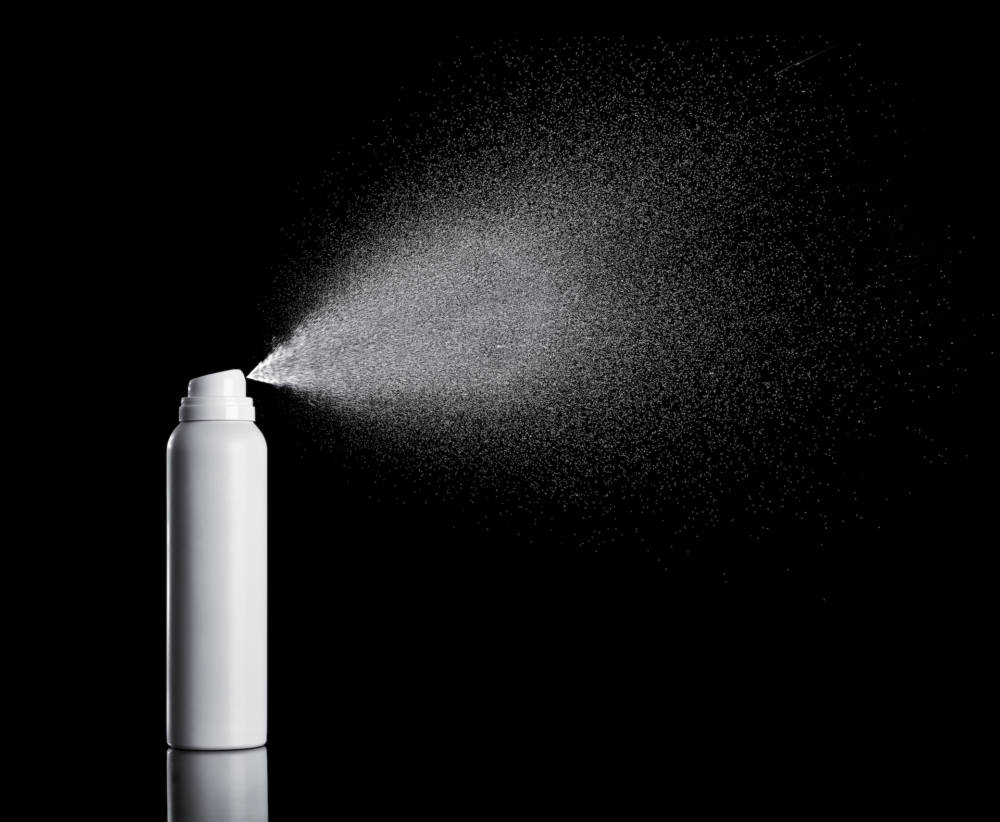
\includegraphics[width=0.8\textwidth]{Plots/deo.jpg}
  \hspace*{12pt}\hbox{\scriptsize {\footnotesize\itshape \href{https://www.stylebook.de/skincare/feinstaub-allergien-atemwege-wie-gesundheitsschaedlich-sind-deo-sprays}
  {stylebook.de}}}
  \vspace*{0.2cm}
  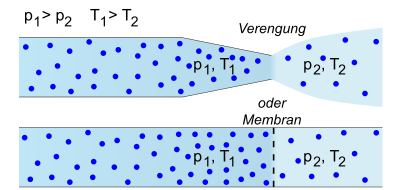
\includegraphics[width=0.8\textwidth]{Plots/ventil.png}
  \hspace*{12pt}\hbox{\scriptsize {\footnotesize\itshape \href{https://lp.uni-goettingen.de/get/text/719}
  {lp.uni-goettingen.de}}}
  \vspace*{0.2cm}
\end{columns}
\end{frame}
\begin{frame}{Detaillierte Aufbau}
  \centering
  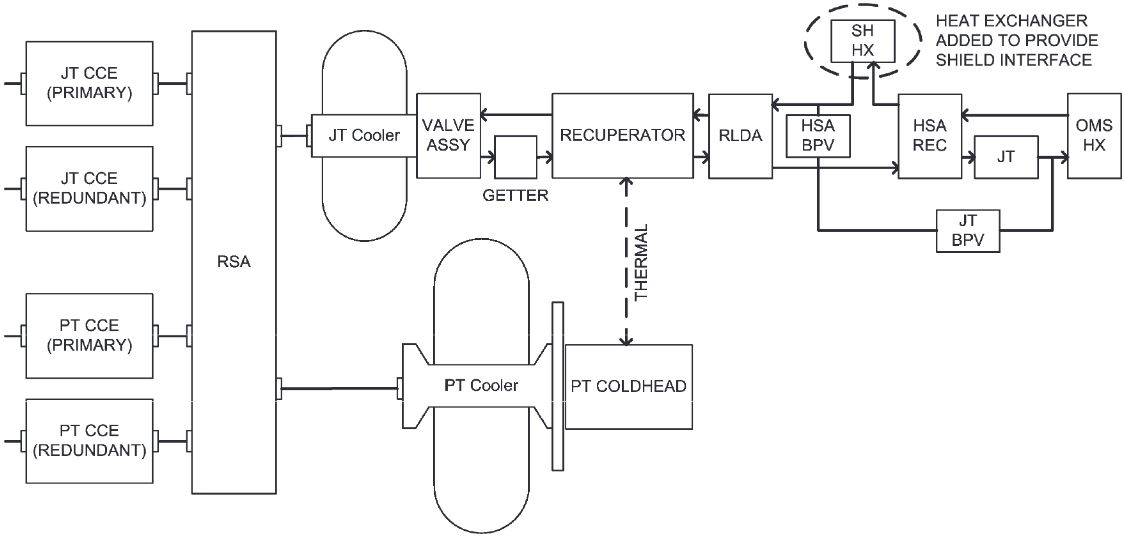
\includegraphics[width=0.8\textwidth]{Plots/diagramm.png}
  \hspace*{12pt}\hbox{\scriptsize {\footnotesize\itshape \href{https://www2.jpl.nasa.gov/adv_tech/coolers/Pub.htm}
  {nasa.gov}}}
\end{frame}
\begin{frame}{Detaillierter Position}
  \centering
  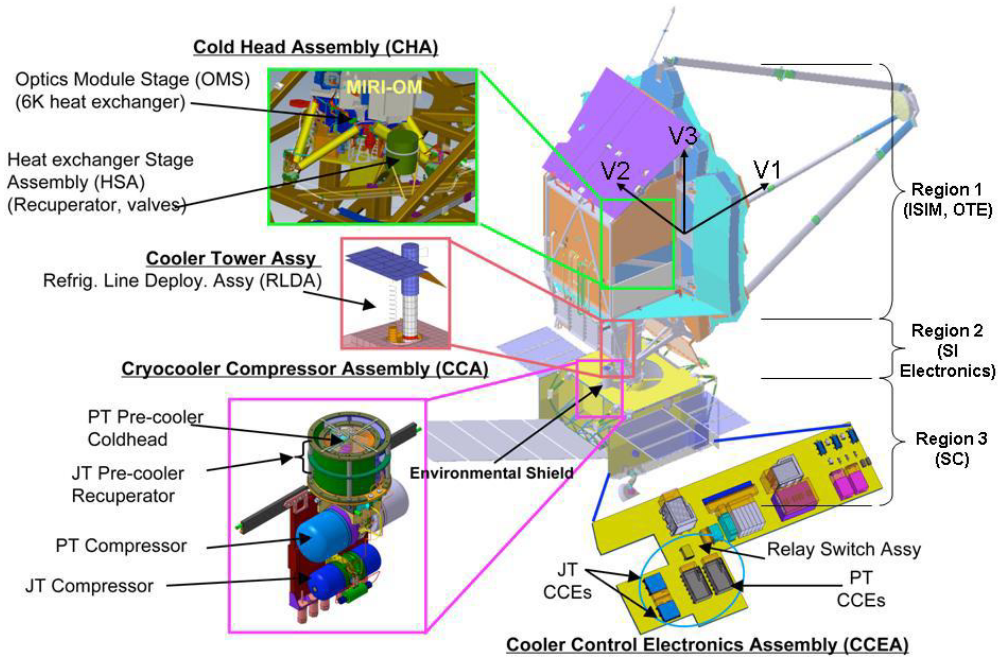
\includegraphics[width=0.7\textwidth]{Plots/realer_Aufbau.png}
  \hspace*{12pt}\hbox{\scriptsize {\footnotesize\itshape \href{http://ircamera.as.arizona.edu/MIRI/}
  {arizona.edu}}}
\end{frame}
\begin{frame}{Pinch Point}
  \centering
  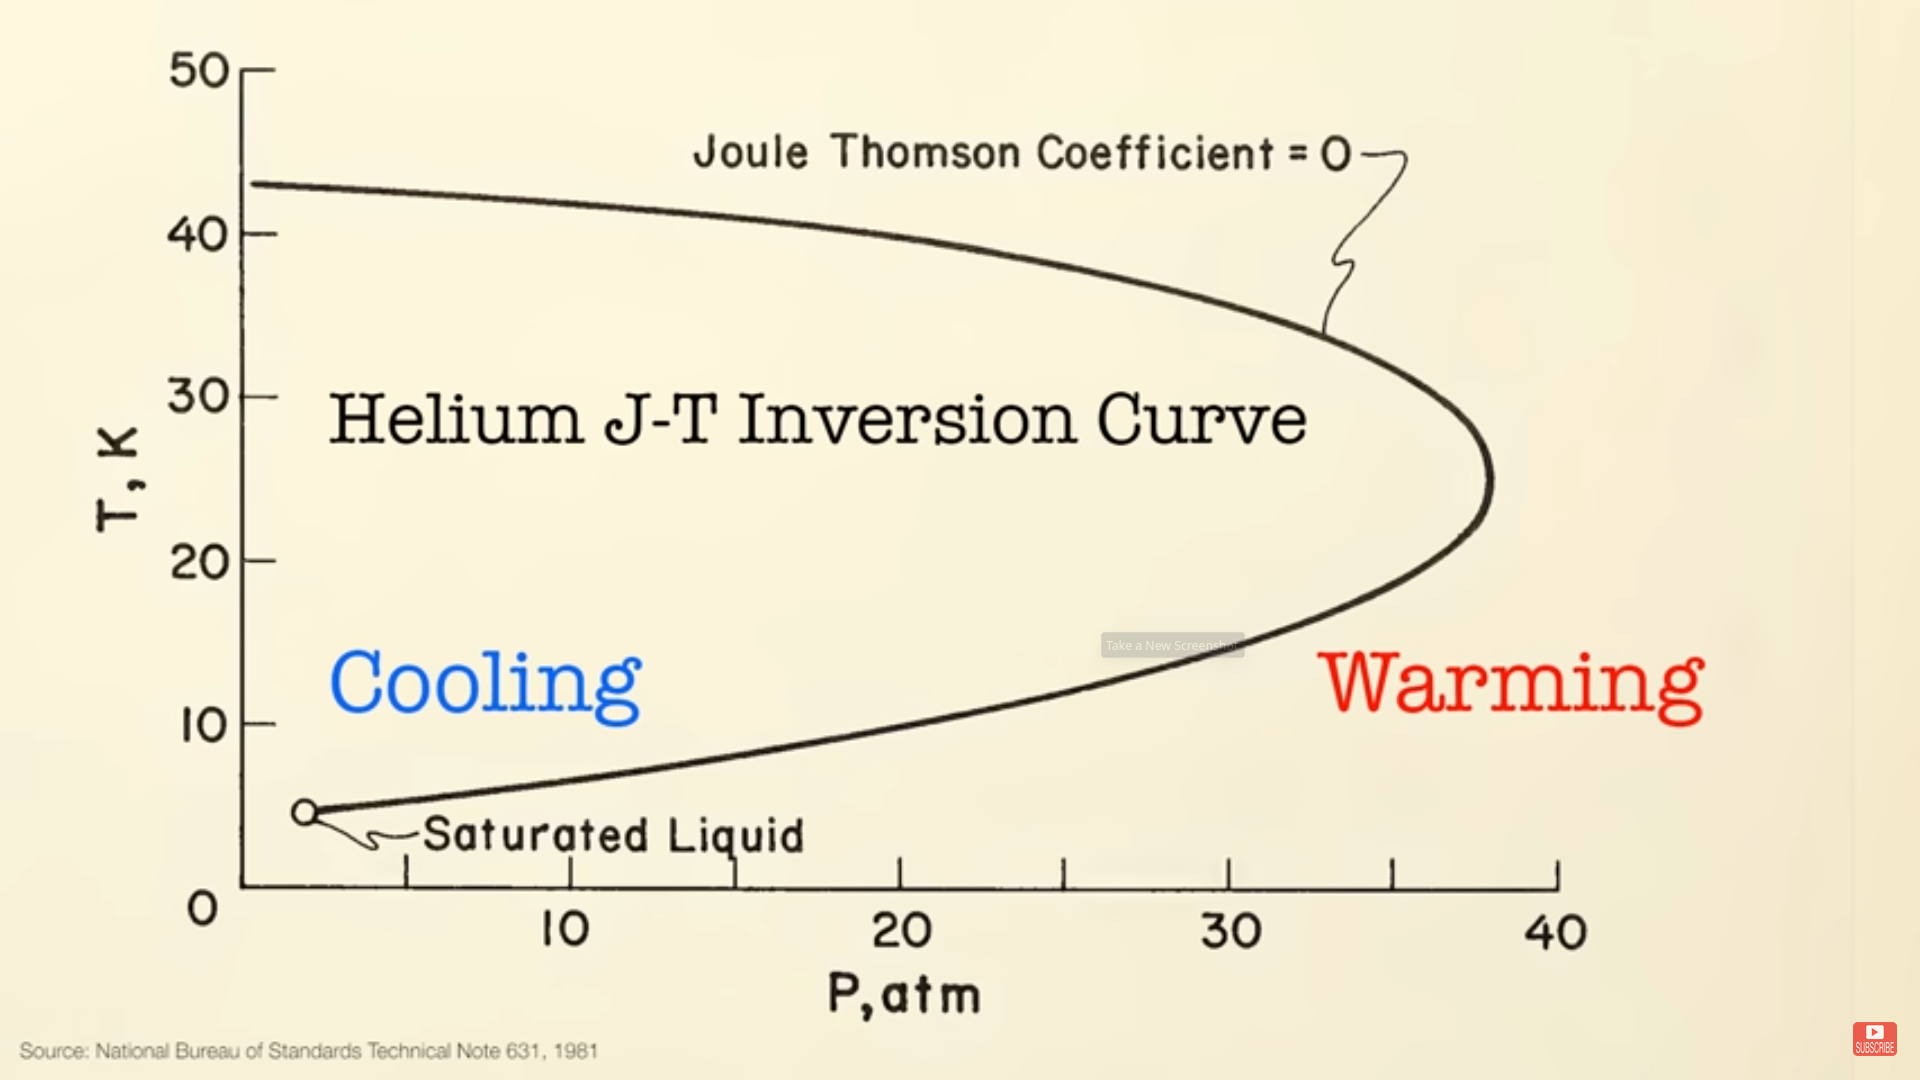
\includegraphics[width=0.4\textwidth]{Plots/jt.png}
  \hspace*{12pt}\hbox{\scriptsize {\footnotesize\itshape \href{https://www.youtube.com/watch?v=FUH61gx149c}
  {youtube.com}}}
  \centering
  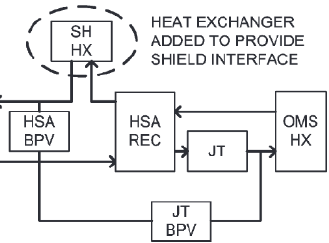
\includegraphics[width=0.3\textwidth]{Plots/zoom.png}
  \hspace*{12pt}\hbox{\scriptsize {\footnotesize\itshape \href{https://www.youtube.com/watch?v=FUH61gx149c}
  {youtube.com}}}
  \vspace*{0.5cm}
  \begin{itemize}
    \item MIRI wird auf etwas weniger als $\qty{15}{\kelvin}$ runtergekühlt mit bypass Ventil
    \item ab dann übernimmt das JT Ventil ("{\color{tugreen}Pinch Point}")
    \item wenn JT Ventil zu früh übernimmt {\color{tugreen}\rightarrow} Erwärwung von MIRI  
  \end{itemize}
\end{frame}
\begin{frame}{Temperaturverlauf}
  \centering
  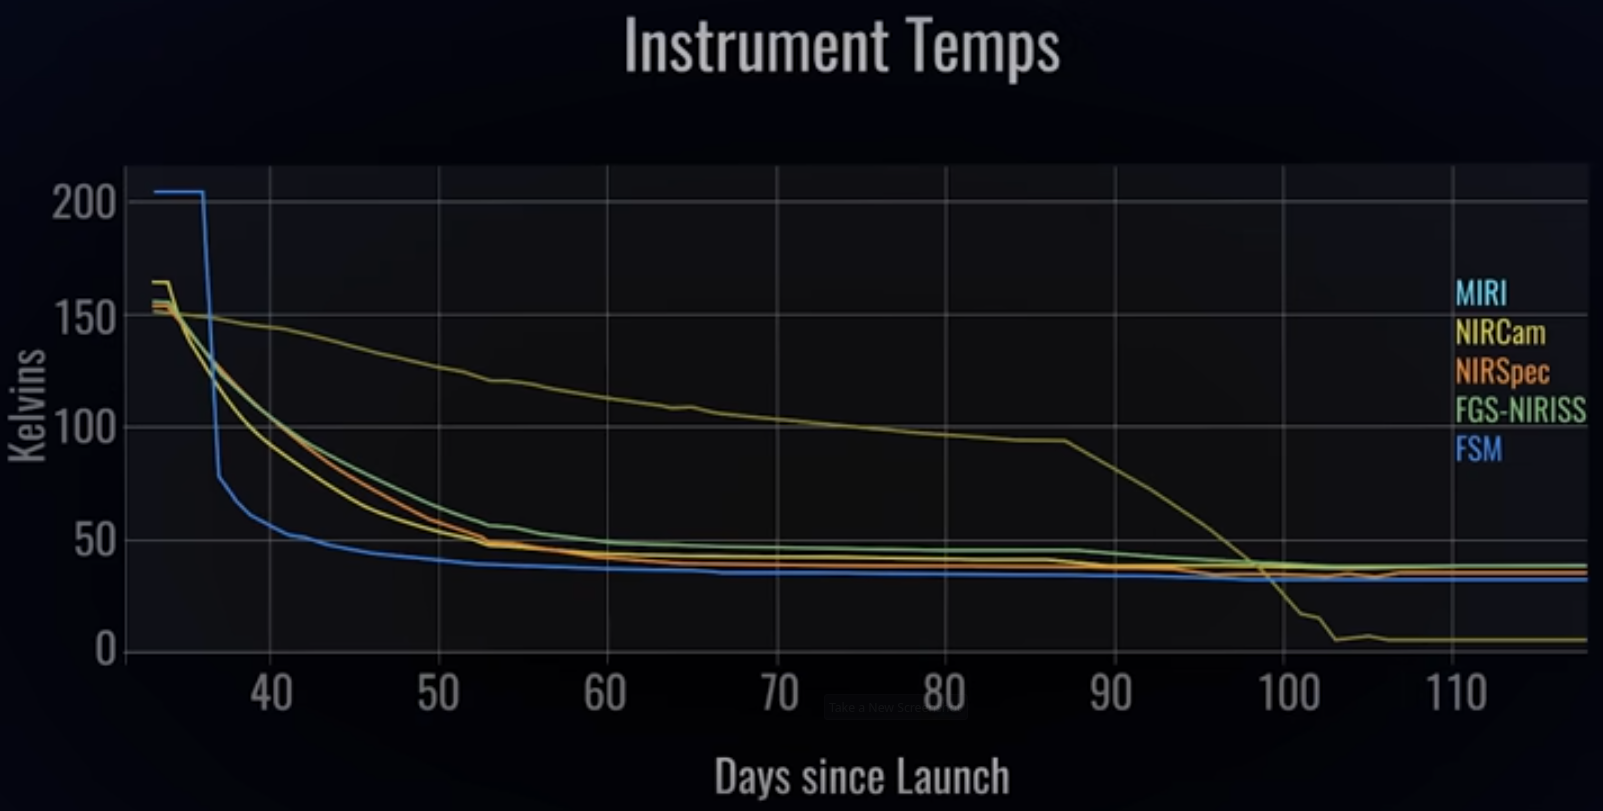
\includegraphics[width=0.8\textwidth]{Plots/temperatur.png}
  \hspace*{12pt}\hbox{\scriptsize {\footnotesize\itshape \href{https://www.youtube.com/watch?v=FUH61gx149c}
  {youtube.com}}}
\end{frame}
\end{document}